\documentclass[aspectratio=169]{beamer}


%%%%%%%%%%%%%%%%%%%%%%%%%%%%%%%%%%%%%%%%%%%%%%%%%%%%%%%%%%%%%%%%%%%%%%%%%%%%%%%%%
% PREAMBLE

% DEFINE VARIABLES
\newcommand{\Lesson}{TEMA EJEMPLO}
\newcommand{\Subject}{Ejemplos, ejemplos, y ejemplos}
\newcommand{\Program}{Inversiones Financieras}
\newcommand{\Professor}{CUNEF Universidad}

% FOOTER WITH LOGO
\setbeamertemplate{footline}{
\hfill
\includegraphics[width=1.2cm]{figs/logo.png}\hspace{13cm}\vspace*{0.5cm}
\insertframenumber \hspace{1cm}
}

% FOOTER WITHOUT LOGO
\newcommand{\NoLogoFootline}{
    \setbeamertemplate{footline}{
    \hfill\vspace*{0.5cm}    
    }
}

% PACKAGES
\usepackage{framed, color}
\definecolor{shadecolor}{rgb}{1,0.9,0.8}
\usepackage[absolute,overlay]{textpos}
\usepackage{graphicx, tikz,xcolor}
\usepackage{multirow, bigstrut,epstopdf}
\usepackage{amsmath,relsize,bigdelim}
\usepackage{hyperref}
\hypersetup{
    colorlinks=true,
    linkcolor=blue,
    filecolor=magenta,      
    urlcolor=cyan,
}
\usepackage[font=tiny]{caption}

\setbeamercolor{block body}{bg=CUNEFGray!20,fg=Front}
\setbeamercolor{block title}{bg=CUNEFOrange,fg=white}

\usetikzlibrary{shapes.geometric, arrows.meta}


% IDENTATION OPTIONS
\setlength{\leftmargini}{1em} % for itemize and enumerate level 1
\setlength{\leftmarginii}{1em} % for itemize and enumerate level 2
\setlength{\leftmarginiii}{1em} % for itemize and enumerate level 3

% COLOR OPTIONS
\definecolor{CUNEFOrange}{RGB}{255, 87, 0}
\definecolor{CUNEFGray}{RGB}{214, 209, 196}
\definecolor{Front}{RGB}{21,31,108}
% BEAMER OPTIONS
\setbeamertemplate{navigation symbols}{}
\setbeamercolor{itemize item}{fg = CUNEFOrange}
\setbeamercolor{itemize subitem}{fg = CUNEFOrange}
\setbeamercolor{itemize subsubitem}{fg = CUNEFOrange}		
\setbeamercolor{enumerate item}{fg = CUNEFOrange}
\setbeamercolor{enumerate subitem}{fg = CUNEFOrange}
\setbeamercolor{enumerate subsubitem}{fg = CUNEFOrange}		
\setbeamercolor{normal text}{fg=Front}

\setbeamercolor{frametitle}{fg=CUNEFOrange}

% NEW TITLE SLIDE
\newcommand{\CUNEFTitleSlide}{\begin{frame}



%\begin{textblock*}{0.1\paperwidth}(0.01\paperwidth,0.01\paperwidth)
%\includegraphics[width=0.3\paperwidth]{Logo_WQU.png}
%\end{textblock*}

\vspace{2em}
%\centering\scriptsize{{\textcolor{CUNEFOrange}{\Lesson}}} \\[1em]
\centering\textbf{{\large\textcolor{CUNEFOrange}{Econometrics 2024/2025}}} \\ [1em]
\centering{\large\textcolor{CUNEFOrange}{}} \\ [1em]
\vspace{0.5em}
\centering{\normalsize\textcolor{CUNEFOrange}{Topic 5: Regression Analysis with Time Series Data}}
\end{frame}}

% NEW SLIDE TEMPLATE
\newcommand{\slide}[2]{\begin{frame}
%\begin{textblock*}{0.1\paperwidth}(0.01\paperwidth,0.01\paperwidth)
%\includegraphics[width=0.15\paperwidth]{Logo_WQU.png}
%\end{textblock*}


\begin{textblock*}{0.87\paperwidth}(0.05\paperwidth,1.2cm)
{\Large\textcolor{CUNEFOrange}{#1}}
\end{textblock*}

\begin{textblock*}{0.87\paperwidth}(0.05\paperwidth,2cm)
#2
\end{textblock*}

\begin{textblock*}{\paperwidth}(0.01\paperwidth,0.95\paperheight)
\noindent\begin{tikzpicture}
%\draw[CUNEFOrange] (0,0) rectangle (0.9\paperwidth,0.8em);
%\draw[CUNEFOrange] (0.9\paperwidth+0.01\paperwidth,0) rectangle (\paperwidth-0.02\paperwidth,0.8em);
%\node[right] at (0,0.4em) {\tiny\textcolor{CUNEFGray}{\Subject\enspace-- \Program\enspace-- \Professor\enspace}};
\end{tikzpicture}
{\tiny\textcolor{CUNEFGray}\thepage}
\end{textblock*}
\end{frame}
}
%%%%%%%%%%%%%%%%%%%%%%%%%%%%%%%%%%%%%%%%%%%%%%%%%%%%%%%%%%%%%%%%%%%%%%%%%%%%%%%%%

% TOC AT BEGINNING OF EACH SECTION
\AtBeginSection[]{
    \begin{frame}<beamer>
    \frametitle{\textcolor{CUNEFOrange}{Outline}}
    \tableofcontents[currentsection]
    \end{frame}
}



\begin{document}

%%%%%%%%%%%%%%%%%%%%%
% Title Page
%%%%%%%%%%%%%%%%%%%%
\NoLogoFootline
{\usebackgroundtemplate{%
  
\includegraphics[width=\paperwidth,height=\paperheight]{figs/title_page.png}}
\CUNEFTitleSlide}

%%%%%%%%%%%%%%%%%%%%%
% Start slides
%%%%%%%%%%%%%%%%%%%%
\setbeamertemplate{footline}{
\hfill
\includegraphics[width=1.2cm]{figs/logo.png}\hspace{13cm}\vspace*{0.5cm}
\insertframenumber \hspace{1cm}
}

\begin{frame}
\frametitle{\textcolor{CUNEFOrange}{Outline}}
   \tableofcontents 
\end{frame}


\section{The nature of time series data}
\frame<beamer>{\frametitle{\textcolor{CUNEFOrange}{The nature of time series data
}}
\begin{itemize}

\item Time series are \textbf{sequences of random variables} (also known as stochastic processes)
\begin{itemize}
   \item One sample is one realized path of the time series out of the many possible paths the stochastic process could have taken. 
\end{itemize}


\item The most distinctive feature of time series data is the temporal ordering of observations; may not be arbitrarily reordered.

\item Time series often exhibit serial correlation: the data is correlated with its own lags. 


\end{itemize}

}

%%%%%%%%%%%%%%%%%%%%%%%%%%

\frame<beamer>{\frametitle{\textcolor{CUNEFOrange}{The nature of time series data
}}

\begin{columns}
    % Left column for the image
    \begin{column}{0.5\textwidth}
        \centering
        \begin{figure}
            \centering
            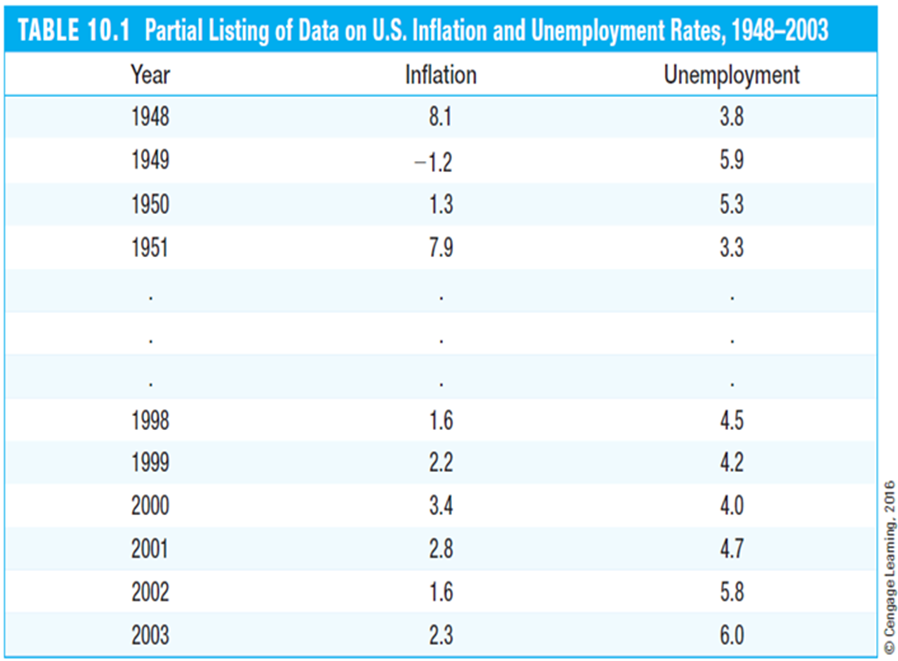
\includegraphics[width=1\linewidth]{figs/time_series_data.png}
        \end{figure}
    \end{column}

    % Right column for the items
    \begin{column}{0.5\textwidth}
        \begin{itemize}
            \item Here, there are only two time series. There may be many more variables whose paths over time are observed simultaneously.

            \item Time series analysis focuses on modeling the dependency of a variable on its own past, and  on the present and past values of other variables.

        \end{itemize}
    \end{column}
\end{columns}


}

%%%%%%%%%%%%%%%%%%%%%%%%%%
\section{Static models
}
\frame<beamer>{\frametitle{\textcolor{CUNEFOrange}{Static models
}}

\begin{itemize}
    \item In static time series models, the current value of one variable is modeled as the result of the current values of explanatory variables.
    \item \textbf{Examples of static model}:

\begin{itemize}
    

\item Return on equity modeled as a function of leverage and liquidity ratios.
\[
        \text{ROE}_t = \beta_0 + \beta_1 \text{Leverage}_t + \beta_2 \text{Liquidity}_t + u_t
        \]

 \item The current stock price determined by current earnings and interest rates.
  \[
        \text{StockPrice}_t = \beta_0 + \beta_1 \text{Earnings}_t + \beta_2 \text{InterestRate}_t + u_t
        \]



  \end{itemize}      
\end{itemize}



}

%%%%%%%%%%%%%%%%%%%%%%%%%%
\section{Finite distributed lag models
}

\frame<beamer>{\frametitle{\textcolor{CUNEFOrange}{
Finite distributed lag models
}}

\begin{itemize}
  \item In finite distributed lag models, the explanatory variables are allowed to influence the dependent variable with a time lag.

\item \textbf{Example for a finite distributed lag model}
    \begin{itemize}
        \item The current sales revenue may depend on advertising expenditures, but the effect of advertising may occur over several periods.
    \end{itemize}
\end{itemize}

\[
\text{Revenue}_t = \alpha_0 + \delta_0 \text{AdSpend}_t + \delta_1 \text{AdSpend}_{t-1} + \delta_2 \text{AdSpend}_{t-2} + u_t
\]

\begin{itemize}
    \item \textbf{Explanation:}
    \begin{itemize}
        \item \(\delta_0\): Effect of current advertising spend.
        \item \(\delta_1\): Effect of last period's advertising spend.
        \item \(\delta_2\): Effect of advertising spend two periods ago.
    \end{itemize}

\end{itemize}

}

%%%%%%%%%%%%%%%%%%%%%%%%%%

\frame<beamer>{\frametitle{\textcolor{CUNEFOrange}{
Finite distributed lag models
}}

\begin{itemize}
    \item Interpretation of the effects in finite distributed lag models
$$
y_t=\alpha_0+\delta_0 z_t+\delta_1 z_{t-1}+\ldots+\delta_q z_{t-q}+u_t
$$

\item  \textbf{Effect of a transitory shock}:
If there is a one time shock in a past period, the dep. variable will change temporarily by the amount indicated by the coefficient of the corresponding lag.
$$
\frac{\Delta y_t}{\Delta z_{t-s}}=\delta_s
$$


\item  \textbf{Effect of permanent shock}:
If there is a permanent shock in a past period, i.e. the explanatory variable permanently increases by one unit, the effect on the dep. variable will be the cumulated effect of all relevant lags. This is a longrun effect on the dependent variable.
$$
\frac{\Delta y_t}{\Delta z_{t-q}}+\ldots+\frac{\Delta y_t}{\Delta z_t}=\delta_1+\ldots+\delta_q
$$

\end{itemize}
}

%%%%%%%%%%%%%%%%%%%%%%%%%%

\frame<beamer>{\frametitle{\textcolor{CUNEFOrange}{
Finite distributed lag models
}}

\begin{columns}
    % Left column for the image
    \begin{column}{0.5\textwidth}
        \begin{figure}
            \centering
            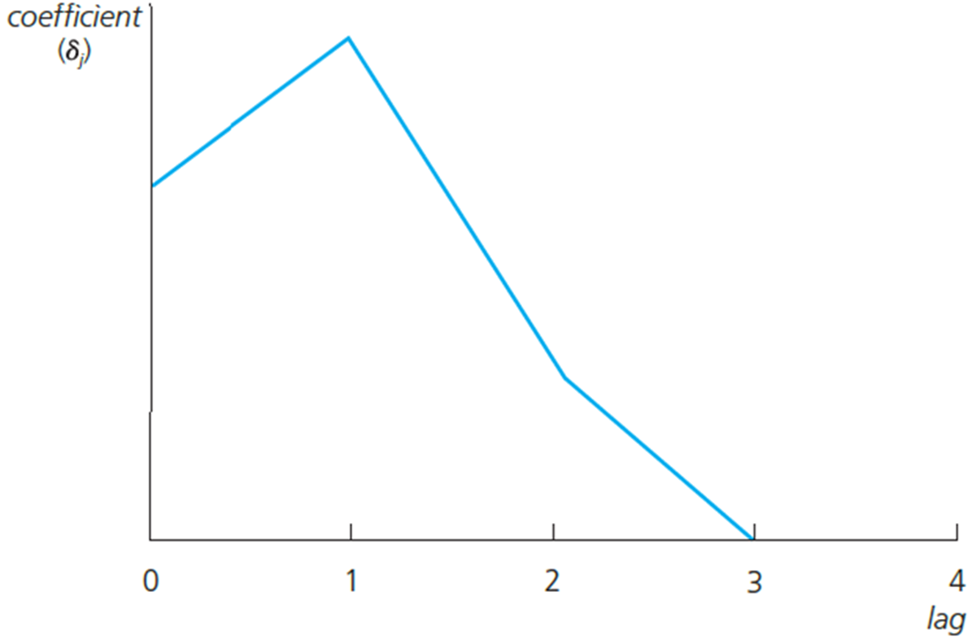
\includegraphics[width=1\linewidth]{figs/lags.png}
        \end{figure}
        
    \end{column}

    % Right column for the items
    \begin{column}{0.5\textwidth}
        \begin{itemize}
            \item The effect is biggest after a lag of one period. After that, the effect vanishes (if the initial shock was transitory).


            \item The long run effect of a permanent shock is the cumulated effect of all relevant lagged effects. It does not vanish (if the initial shock is a permanent one).


        \end{itemize}
    \end{column}
\end{columns}

}

%%%%%%%%%%%%%%%%%%%%%%%%%%
\section{Properties of OLS under classical assumptions}
\frame<beamer>{\frametitle{\textcolor{CUNEFOrange}{
Properties of OLS under classical assumptions}}

\begin{itemize}
    \item \textbf{Assumption TS.1 (Linear in parameters)}: The time series involved obey a linear relationship. The stochastic processes $y_t, x_{t 1}, \ldots$, $x_{t k}$ are observed, the error process $u_t$ is unobserved. The definition of the explanatory variables is general, e.g. they may be lags or functions of other explanatory variables.
    $$
y_t=\beta_0+\beta_1 x_{t 1}+\beta_2 x_{t 2}+\ldots+\beta_k x_{t k}+u_t
$$

\item \textbf{Assumption TS.2 (No perfect collinearity)}: In the sample (and therefore in the underlying time series process), no independent variable is constant nor a perfect linear combination of the others
\end{itemize}

}

%%%%%%%%%%%%%%%%%%%%%%%%%%

\frame<beamer>{\frametitle{\textcolor{CUNEFOrange}{
Properties of OLS under classical assumptions}}

\begin{itemize}
    \item \textbf{Assumption TS.3 (Zero conditional mean)}: The mean value of the unobserved factors is uncorrelated to the values of the explanatory variables in all periods
    $$
E\left(u_t \mid \mathrm{X}\right)=0, t=1,2, \ldots, n
$$

\item Discussion of assumption TS.3
\begin{itemize}
    \item \textbf{Exogeneity}: The mean of the error term is uncorrelated to the explanatory variables of the same period
    $$
E\left(u_t \mid \mathbf{x}_t\right)=0
$$

\item Strict exogeneity: The mean of the error term is uncorrelated to the values of the explanatory variables of all periods
$$
E\left(u_t \mid \mathbf{X}\right)=0
$$

\item Strict exogeneity is stronger than contemporaneous exogeneity


\end{itemize}

\end{itemize}

}

%%%%%%%%%%%%%%%%%%%%%%%%%%

\frame<beamer>{\frametitle{\textcolor{CUNEFOrange}{
Properties of OLS under classical assumptions}}

\begin{itemize}
    \item \textbf{Theorem (Unbiasedness of OLS)}: 
    $$
T S .1-T S .3 \Rightarrow E\left(\widehat{\beta}_j\right)=\beta_j, \quad j=0,1, \ldots, k
$$

\item \textbf{Assumption TS.4 (Homoskedasticity)}: The volatility of the errors must not be related to the explanatory variables in any of the periods
$$
\operatorname{Var}\left(u_t \mid \mathrm{X}\right)=\operatorname{Var}\left(u_t\right)=\sigma^2, t=1,2, \ldots, n
$$
In the time series context, homoskedasticity may also be easily violated, e.g. if the volatility of the dep. variable depends on regime changes.


\end{itemize}


}

%%%%%%%%%%%%%%%%%%%%%%%%%%

\frame<beamer>{\frametitle{\textcolor{CUNEFOrange}{
Properties of OLS under classical assumptions}}


\begin{itemize}
    \item \textbf{Assumption TS.5 (No serial correlation)}: Conditional on the explanatory variables, the unobserved factors must not be correlated over time
    $$
\operatorname{Corr}\left(u_t, u_s \mid \mathbf{X}\right)=0, t \neq s
$$

\item Discussion of assumption TS.5
\begin{itemize}
    \item Why was such an assumption not made in the cross-sectional case?
\item The assumption may easily be violated if, conditional on knowing the values of the indep. variables, omitted factors are correlated over time.
\item The assumption may also serve as substitute for the random sampling assumption if sampling a cross-section is not done completely randomly.
\item In this case, given the values of the explanatory variables, errors have to be uncorrelated across cross-sectional units (e.g. states).

\end{itemize}

\end{itemize}

}

%%%%%%%%%%%%%%%%%%%%%%%%%%

\frame<beamer>{\frametitle{\textcolor{CUNEFOrange}{
Properties of OLS under classical assumptions}}

\begin{itemize}
    \item \textbf{Theorem (OLS sampling variances)}: Under assumptions TS.1 – TS.5:
    $$
\operatorname{Var}\left(\widehat{\beta}_j \mid \mathbf{X}\right)=\frac{\sigma^2}{S S T_j\left(1-R_j^2\right)}, \quad j=1, \ldots, k
$$
The conditioning on the values of the explanatory variables is not easy to understand. It effectively means that, in a finite sample, one ignores the sampling variability coming from the randomness of the regressors. This kind of sampling variability will normally not be large (because of the sums).

\item \textbf{Theorem (Unbiased estimation of the error variance)}: Under assumptions TS.1 – TS.5:
$$
E\left(\widehat{\sigma}^2\right)=\sigma^2
$$


\end{itemize}


}

%%%%%%%%%%%%%%%%%%%%%%%%%%

\frame<beamer>{\frametitle{\textcolor{CUNEFOrange}{
Properties of OLS under classical assumptions}}


\begin{itemize}
    \item \textbf{Theorem (Gauss-Markov Theorem)}: Under assumptions TS.1 – TS.5, the OLS estimators have the minimal variance of all linear unbiased estimators of the regression coefficients.

\item \textbf{Assumption TS.6 (Normality)}: 
$$
u_t \sim \operatorname{Normal}\left(0, \sigma^2\right)
$$

\item \textbf{Theorem (Normal sampling distributions)}: Under assumptions TS.1 – TS.6, the OLS estimators have the usual normal distribution (conditional on X). The usual $F$ and $t$-tests are valid.



\end{itemize}


}

%%%%%%%%%%%%%%%%%%%%%%%%%%

\frame<beamer>{\frametitle{\textcolor{CUNEFOrange}{
Properties of OLS under classical assumptions: The Static Phillips curve}}

\begin{itemize}
    \item \textbf{Example: Static Phillips curve}
$$
\begin{aligned}
& \widehat{inf}_t=\underset{(1.72)}{1.42}+\underset{(.289)}{.468} \text {unem}_t \\
& n=49, R^2=.053
\end{aligned}
$$
Contrary to theory, the estimated Phillips Curve does not suggest a trade-off between inflation and unemployment!

\item \textbf{Discussion on Assumption TS.1 (Linear in parameters)}: The error term contains factors such as monetary shocks, income/demand shocks, oil price shocks, supply shocks, or exchange rate shocks.


    
\end{itemize}

}

%%%%%%%%%%%%%%%%%%%%%%%%%%

\frame<beamer>{\frametitle{\textcolor{CUNEFOrange}{
Properties of OLS under classical assumptions: The Static Phillips curve}}

\begin{itemize}
    \item \textbf{Discussion on Assumption TS.2 (No perfect collinearity)}:  A linear relationship might be restrictive, but it should be a good approximation. Perfect collinearity will seldomly be a problem in practice. 

    \item \textbf{Discussion on Assumption TS.3 (Zero conditional mean)}: 
$$
E\left(u_t \mid \text { unem }_1, \ldots, \text { unem }_n\right)=0 \longleftarrow \text { Easily violated }
$$
$$
\text {unem}_{t-1} \uparrow \rightarrow u_t \downarrow \begin{aligned}
& \text { For example, past unemployment shocks may lead to } \\
& \text { future demand shocks which may dampen inflation }
\end{aligned}
$$
$$
u_{t-1} \uparrow \rightarrow \text {unem}_t \uparrow \begin{aligned}
& \text { For example, an oil price shock means more inflation } \\
& \text { and may lead to future increases in unemployment }
\end{aligned}
$$
\end{itemize}

}

%%%%%%%%%%%%%%%%%%%%%%%%%%

\frame<beamer>{\frametitle{\textcolor{CUNEFOrange}{
Properties of OLS under classical assumptions: The Static Phillips curve}}

\begin{itemize}
    \item \textbf{Discussion on Assumption TS.4 (Homoskedasticity)}:
$$
\operatorname{Var}\left(u_t \mid \text { unem }_1, \ldots, \text { unem }_n\right)=\sigma^2
$$
Assumption is violated if monetary policy is more ``nervous'' in times of high unemployment

\item D\textbf{iscussion on Assumption TS.5 (No serial correlation)}: 
$$
\operatorname{Corr}\left(u_t, u_s \mid \text { unem }_1, \ldots, \text { unem }_n\right)=0
$$
Assumption is violated if exchange rate influences persist over time (they cannot be explained by unemployment)



\end{itemize}

}

%%%%%%%%%%%%%%%%%%%%%%%%%%

\frame<beamer>{\frametitle{\textcolor{CUNEFOrange}{
Properties of OLS under classical assumptions: The Static Phillips curve}}

\begin{itemize}
    \item \textbf{Discussion on Assumption TS.6 (Normality)}: 
    $$
u_t \sim \operatorname{Normal}\left(0, \sigma^2\right) \longleftarrow \text { Questionable? }
$$
\end{itemize}


}

%%%%%%%%%%%%%%%%%%%%%%%%%%
\section{Using dummy explanatory variables in time series}
\frame<beamer>{\frametitle{\textcolor{CUNEFOrange}{
Using dummy explanatory variables in time series
}}

\begin{itemize}
   \item Consider a model where the quarterly growth rate of company revenue is influenced by seasonal promotions and significant market events.
   \[
\widehat{\text{RevenueGrowth}}_t = 5.67 + 2.45 \text{Promo}_t - 1.83 \text{Recession}_t - 3.12 \text{NewRegulation}_t
\]
\[
n = 40, \ R^2 = .65
\]
$NewRegulation$ is a dummy variable that takes value 1 after the introduction of a new regulation. $Recession$ is a dummy variable that takes value 1 during recession times.


        \item Revenue growth is negatively impacted during recession periods (\(\text{Recession}_t\)).
        \item The introduction of new regulations (\(\text{NewRegulation}_t\)) has a  negative effect on growth.
\end{itemize}


}

%%%%%%%%%%%%%%%%%%%%%%%%%%%%%%%%%%%%%%
\section{Time series with trends}
\frame<beamer>{\frametitle{\textcolor{CUNEFOrange}{
Time series with trends
}}

Example for a time series with a linear upward trend:
\begin{figure}
    \centering
    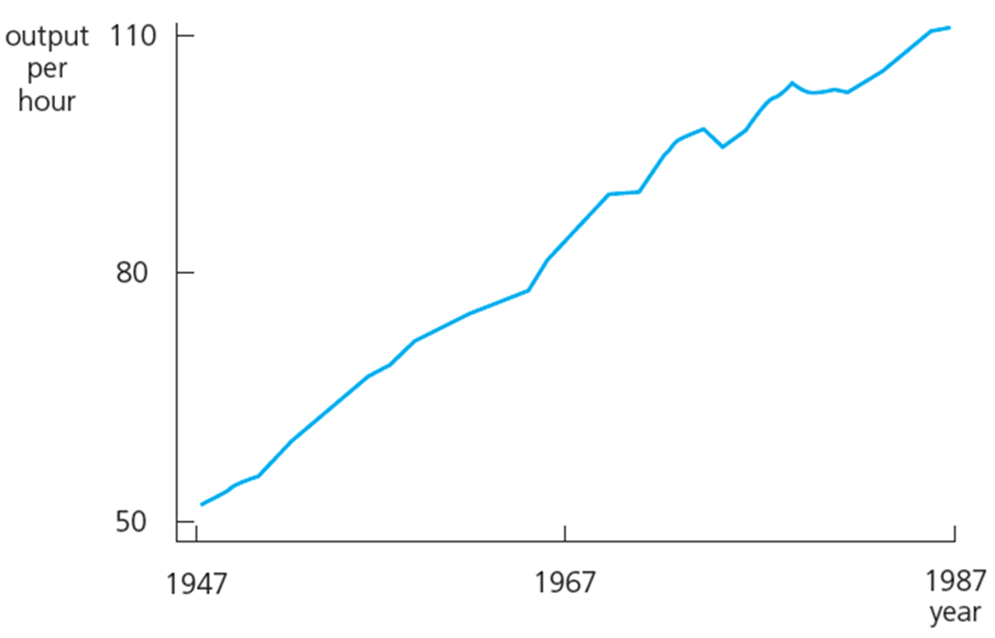
\includegraphics[width=0.7\linewidth]{figs/trend.png}
\end{figure}


}

%%%%%%%%%%%%%%%%%%%%%%%%%%%%%%

\frame<beamer>{\frametitle{\textcolor{CUNEFOrange}{
Time series with trends
}}

\begin{itemize}
   \item \textbf{Modelling a linear time trend}
   $$
y_t=\alpha_0+\alpha_1 t+e_t \quad \Leftrightarrow \quad E\left(\Delta y_t\right)=E\left(y_t-y_{t-1}\right)=\alpha_1
$$

$\Delta y_t / \Delta t=\alpha_1 \longleftarrow \begin{aligned} & \text { Abstracting from random deviations, the dependent } \\ & \text { variable increases by a constant amount per time unit }\end{aligned}$
$E\left(y_t\right)=\alpha_0+\alpha_1 t \longleftarrow \begin{aligned} & \text { Alternatively, the expected value of the dependent } \\ & \text { variable is a linear function of time }\end{aligned}$


\end{itemize}


}


%%%%%%%%%%%%%%%%%%%%%%%%%%%%%%

\frame<beamer>{\frametitle{\textcolor{CUNEFOrange}{
Time series with trends
}}

\begin{itemize}
   \item \textbf{Modelling an exponential time trend}
$$
\log \left(y_t\right)=\alpha_0+\alpha_1 t+e_t \quad \Leftrightarrow \quad E\left(\Delta \log \left(y_t\right)\right)=\alpha_1
$$
$$
\left(\Delta y_t / y_t\right) / \Delta t=\alpha_1
$$
Abstracting from random deviations, the dependent variable increases by a constant \textbf{percentage} per time unit
\begin{figure}
    \hfill
    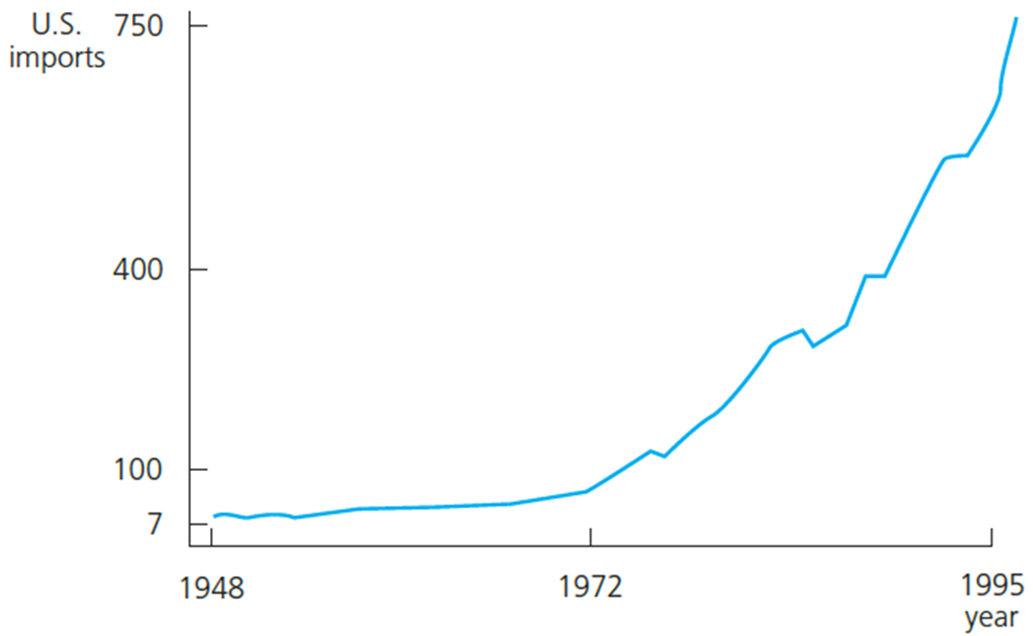
\includegraphics[width=0.5\linewidth]{figs/exp_trend.png}
\end{figure}


\end{itemize}


}


%%%%%%%%%%%%%%%%%%%%%%%%%%%%%%


\frame<beamer>{\frametitle{\textcolor{CUNEFOrange}{
Time series with trends
}}

\textbf{Using trending variables in regression analysis}

\begin{itemize}
   \item If trending variables are regressed on each other, a spurious relationship may arise if the variables are driven by a common trend.
\item In this case, it is important to include a trend in the regression.

\item \textbf{Example}: Housing investment and prices
$$
\begin{aligned}
& \widehat{\log(\text{invpc})}=-\underset{(.043)}{.550}+\underset{(.382)}{1.241} \log (\text{price}) \\
& n=42, R^2=.208
\end{aligned}
$$
It looks as if investment and prices are positively related!

\end{itemize}


}


\frame<beamer>{\frametitle{\textcolor{CUNEFOrange}{
Time series with trends
}}

\textbf{Using trending variables in regression analysis}

\begin{itemize}
   \item Let's add to the regression a time trend variable ($t=1,2,3,....,42$) to the regression:
\[
\begin{aligned}
& \widehat{\log(\text{invpc})} = -\underset{(1.36)}{0.913} - \underset{(0.679)}{0.381} \log(\text{price}) + \underset{(0.0035)}{0.0098}t \\
& n = 42, \ R^2 = 0.341
\end{aligned}
\]
There is no significant relationship between price and investment anymore!

\item When should a trend be included?

\begin{itemize}
    \item If the dependent variable displays an obvious trending behavior.
    \item If both the dependent and some independent variables have trends.
    \item If only some of the independent variables have trends; their effect on the dependent variable may only be visible after a trend has been subtracted.
\end{itemize}

\end{itemize}


}


%%%%%%%%%%%%%%%%%%%%%%%%%%%%%%

\frame<beamer>{\frametitle{\textcolor{CUNEFOrange}{
Time series with trends
}}

\begin{itemize}
    \item \textbf{A detrending interpretation of regressions with a time trend}
\begin{itemize}
    \item  It turns out that the OLS coefficients in a regression including a trend are the same as the coefficients in a regression without a trend but where all the variables have been detrended before the regression.
\item  This follows from the general interpretation of multiple regressions.
\end{itemize}
\item \textbf{Computing R-squared when the dependent variable is trending}

\begin{itemize}
\item Due to the trend, the variance of the dependent variable will be overstated.
\item It is better to first detrend the dependent variable and then run the regression on all the independent variables (plus a trend if they are trending as well).
\item The R -squared of this regression is a more adequate measure of fit.
\end{itemize}
\end{itemize}
}


%%%%%%%%%%%%%%%%%%%%%%%%%%%%%%%%%%%%%%%%%5
\section{Modelling seasonality in time series}
\frame<beamer>{\frametitle{\textcolor{CUNEFOrange}{
Modelling seasonality in time series}}

\begin{itemize}
    \item A simple method is to include a set of \textbf{seasonal dummies:}
    $$
\begin{aligned}
y_t= & \beta_0+\delta_1 \text { feb }_t+\delta_2 \text { mar }_t+\delta_3 \text { apr }_t+\ldots+\delta_{11} \operatorname{dec}_t \\
& +\beta_1 x_{t 1}+\beta_2 x_{t 2}+\ldots+\beta_k x_{t k}+u_t 
\end{aligned}
$$
where $\text{feb}_t=1$ if observation is from February, 0 otherwise.

\item Similar remarks apply as in the case of deterministic time trends:
\begin{itemize}
    \item The regression coefficients on the explanatory variables can be seen as the result of first deseasonalizing the dep. and the explanatory variables.
\item  An R-squared that is based on first deseasonalizing the dependent variable may better reflect the explanatory power of the explanatory variables.
\end{itemize}



\end{itemize}
}


%%%%%%%%%%%%%%%%%%%%%
% Back Page
%%%%%%%%%%%%%%%%%%%%
\NoLogoFootline
{\usebackgroundtemplate{%

\includegraphics[width=\paperwidth,height=\paperheight]{figs/back_page.png}}
\slide{}{}}

\end{document}